% APJ Reference: http://aas.org/journals/authors/common_instruct#_Toc2

\documentclass[iop]{emulateapj}
% \documentclass[12pt,preprint]{aastex}


% Define the sun symbol for use with solar mass
% \newcommand{\Sun}{\odot}
\newcommand{\vect}[1]{\boldsymbol{#1}}
% \usepackage{amssymb}
%\usepackage{xfrac}
% \usepackage{amsmath}
\usepackage{natbib}
\usepackage{footnote}
% \usepackage{multirow}
% \usepackage{array}
% \usepackage[lofdepth,lotdepth]{subfig}
%\usepackage{todonotes}

%\newcommand{\TODO}[1]{\todo[inline]{#1}}
\usepackage{float}

% \newcolumntype{x}[1]{%
% >{\centering\hspace{0pt}}p{#1}}%


\bibliographystyle{apj}

\shortauthors{Brenner}
\shorttitle{Characterizing stellar phenomena with fractals and multifractals}

%--------------------
%	Begin document
%--------------------
\begin{document}
%
\title{Fractal and Multifractal Analysis as Tools to Characterize Supernovae and Molecular Clouds}
%
\author{Samuel Brenner\altaffilmark{1}}
\email{samuel.e.brenner@gmail.com}
%\author{Tomasz Plewa\altaffilmark{1}}
%\email{tplewa@fsu.edu}
%
%\author{Andrzej Odrzwolek\altaffilmark{2}}
%\email{andrzej's email}
%
\altaffiltext{1}{Young Scholars Program, Florida State University}
%
%
%
%--------------------
%	Begin Abstract
%--------------------
\begin{abstract}
\end{abstract}
%
%
%
%--------------------
%	Begin keywords
%--------------------
\keywords{supernovae, fractals, multifractals}
%
%
%
%--------------------
%	Begin Body
%--------------------

\section{Introduction}
Many physical phenomena cannot be characterized by the idealizations of Euclidean geometry alone; they exhibit ``roughness'' of morphology. That is, they have a detailed structure at any arbitrarily small size scale (see \cite{Falconer2003}). We can quantify this roughness with the concept of a fractal dimension, which---just like the Euclidean dimension---tells how some figure fills a space, so that a rougher figure would tend to have a higher fractal dimension than a smooth one. Multifractal analysis extends this paradigm of a fractal dimension by permitting us to examine how those fractal characteristics themselves change with scale; in fact, they may even be fractal themselves. In this paper, we detail the application of fractal geometry to flame fronts in exploding white dwarfs and then analyze the multifractal characteristics of star-forming molecular clouds.

\subsection{Fractal analysis of Type Ia supernova flame fronts}
The accepted model for a Type Ia supernova is a white dwarf that accumulates mass from a binary companion until it reaches a mass so large that the compression and heating of the core causes heavier elements to begin fusing. This fusion gives off even more heat, starting a cascade of fusion reactions: a subsonic thermonuclear flame front. This front spreads rapidly throughout the star and causes the explosion of the white dwarf.

The morphology of the expanding flame front can be dramatically affected by multiple types of perturbations. \cite{Landau1959} showed that the flame surface is subject to Landau-Darrieus instability in which the front is convoluted due to thermal expansion across the flame front. It is also widely established \citep{Khokhlov} that Rayleigh-Taylor instability, in which a denser fluid pushes through a less-dense one under the influence of a gravitational field, can contort the deflagration front in a supernova. These wrinkles on the surface of the flame front increase the front's effective surface area, and because the flame speed is proportional to the flame's surface area, the convolution of the surface can influence the rate at which the flame consumes the stellar material. Thus, characterizing the shape of the flame front plays a crucial part in characterizing the supernova explosion process as a whole.

\begin{figure}[ht]
	\begin{center}
	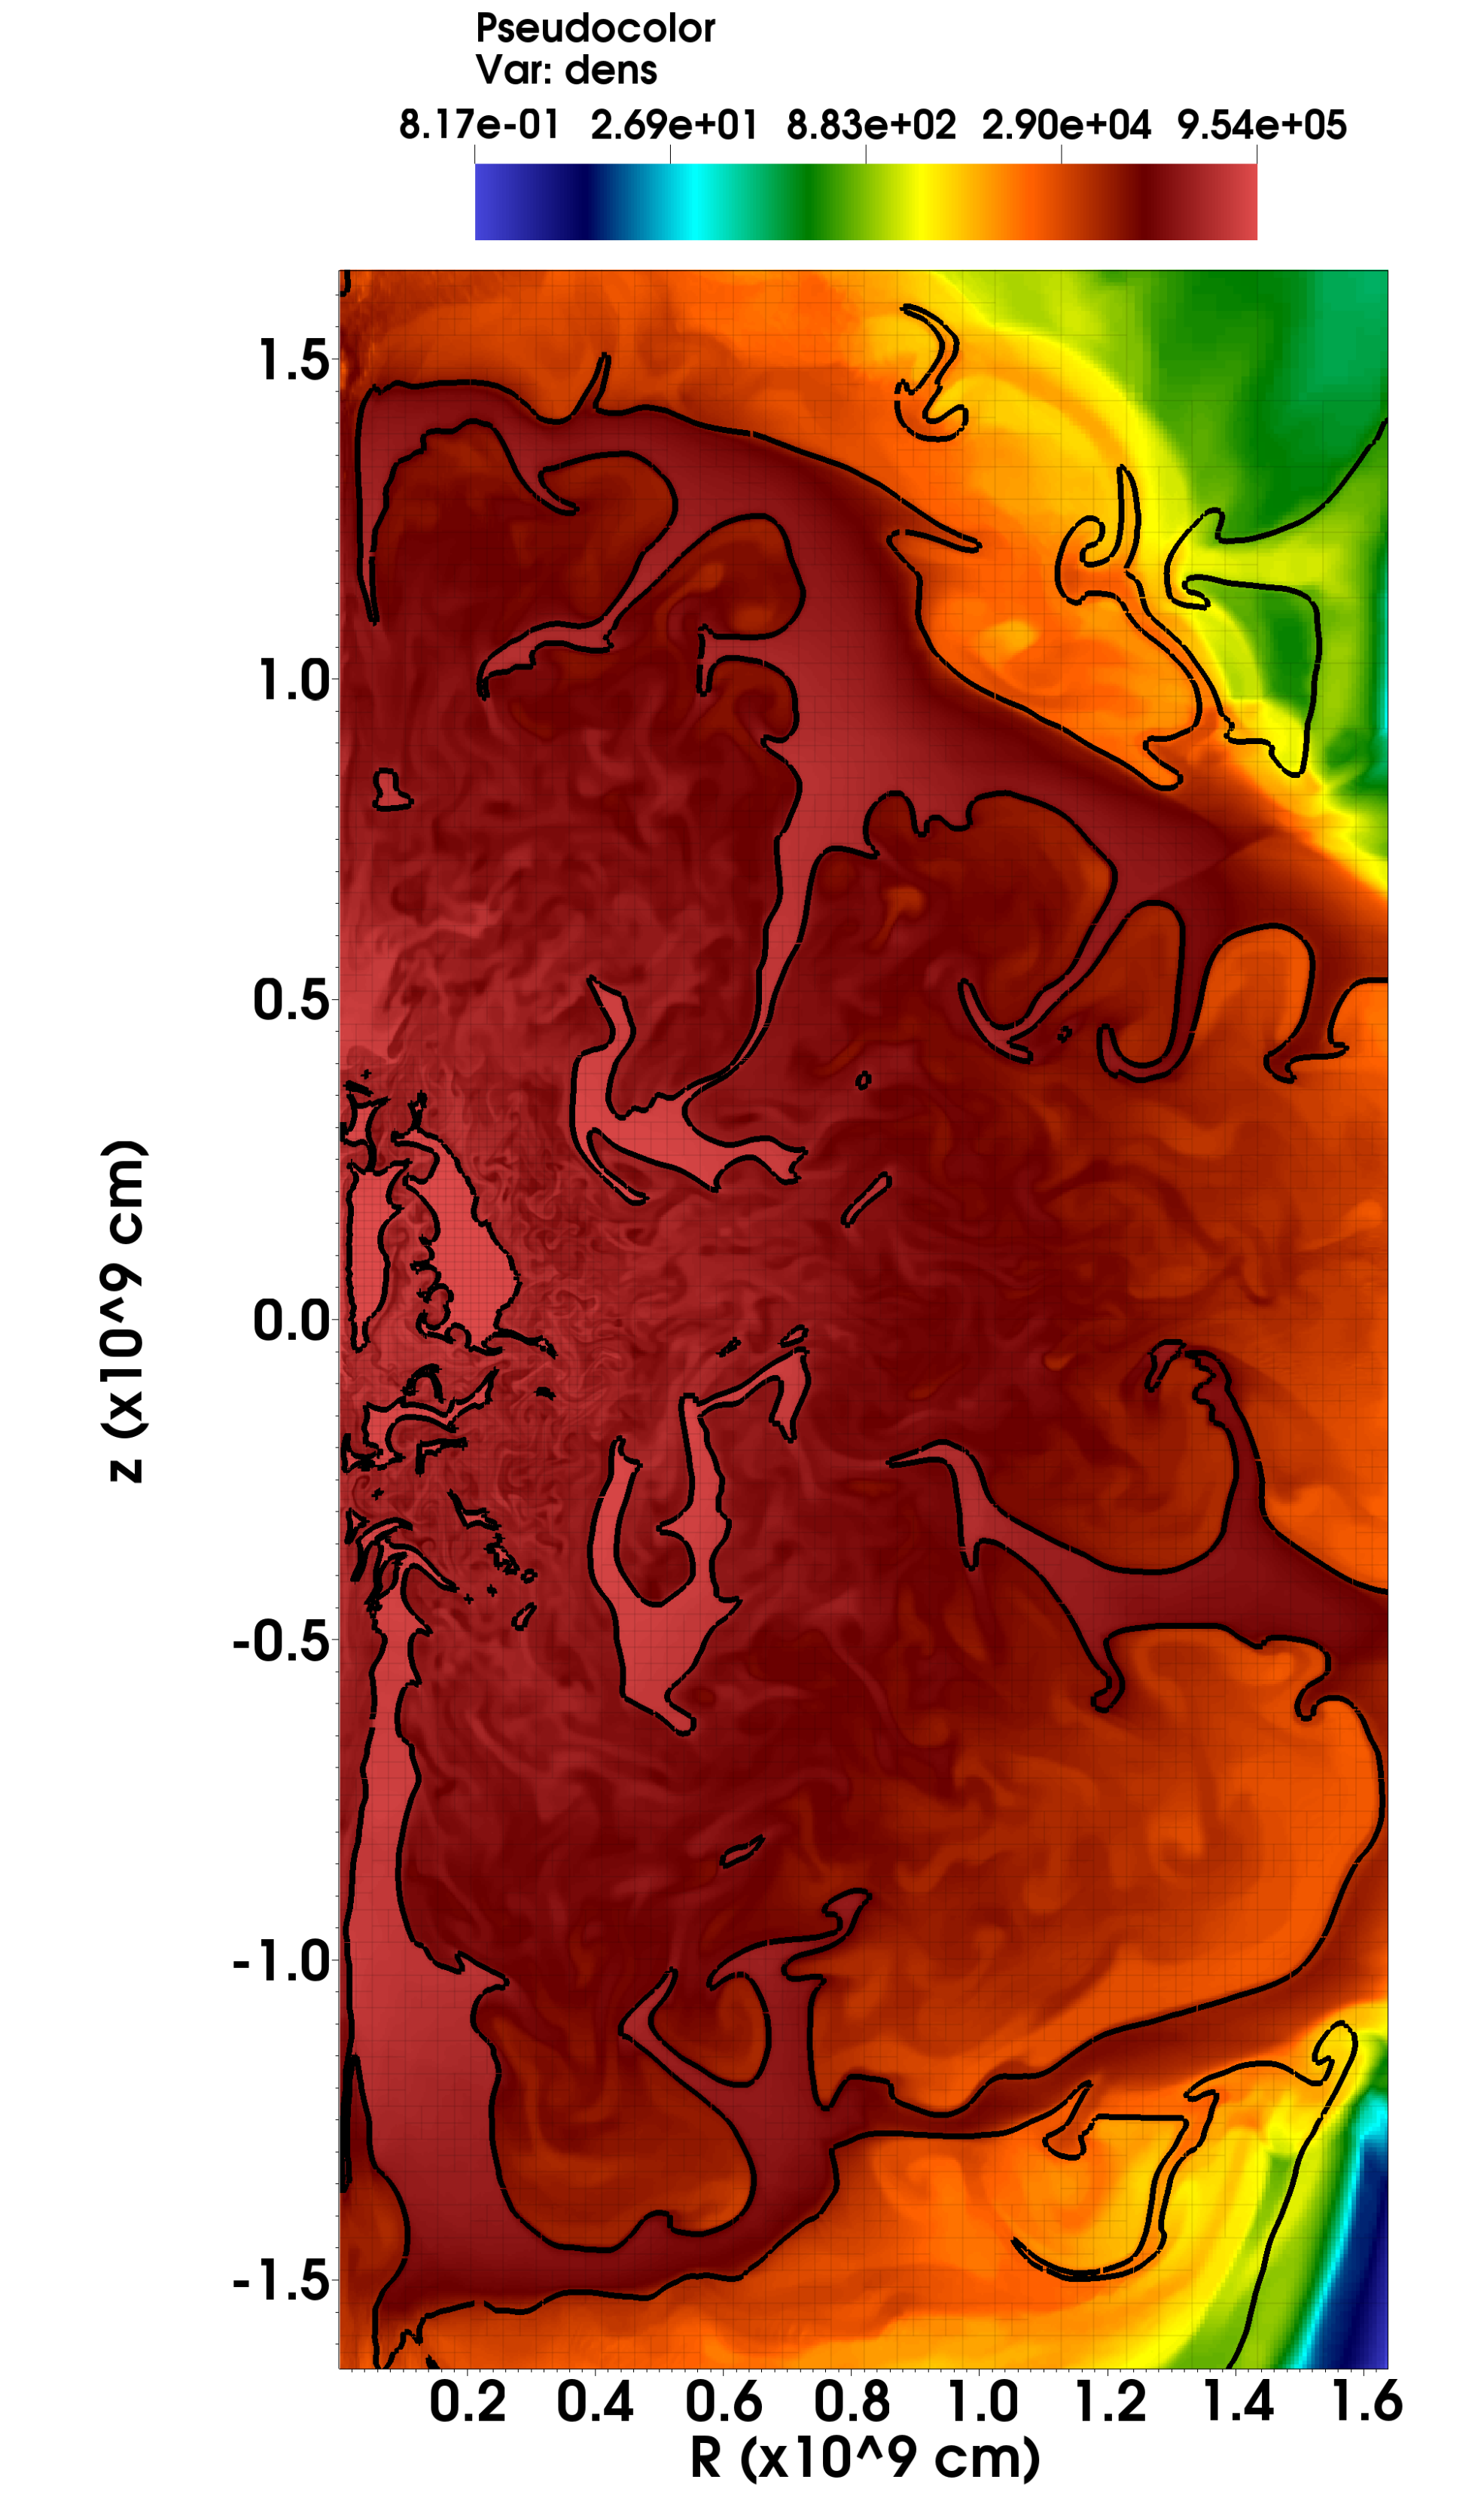
\includegraphics[width=0.45\textwidth,clip=true]{Graphics/n7d1r10t15b0011_cropped.png}
	\caption{Simulation of Type Ia supernova in a white dwarf. The contour of the flame front is highlighted in black. False color indicates density in $\mathrm{g/cm^3}$.
	\label{f:flamefrontwithcontour}}
	\end{center}
	\end{figure} 

The convolutions of the surface of a turbulent front can be viewed within the framework of fractal geometry, as was proposed by \cite{Mandelbrot1975} and further developed by \cite{Timmes1994}. In particular, Timmes showed that the final effective speed $v_{eff}$ of the flame front can be expressed as a function of its fractal dimension:
\begin{equation} 
	v_{eff} = v_{lam} \left(\frac{l_{min}}{l_{max}}\right)^{2 - D},
\end{equation}
where $v_{lam}$ is the laminar flame speed (that is, the speed of the flame in the absence of perturbations), $l_{min}$ is the minimum length scale at which the turbulence takes place, $l_{max}$ is the maximum length scale at which the turbulence takes place, and $ D $ is the fractal dimension of the flame front.

In \textsection \ref{Methods}, we discuss the implemention of a method to perform fractal analysis of a supernova flame front. The results are discussed in \textsection \ref{Results}, and the implications of our findings are discussed in \textsection \ref{Discussion}.

\subsection{Multifractal analysis of star-forming molecular clouds}
Clouds often form in the interstellar medium (ISM), and turbulence like that caused by stellar winds can create structures which under their own gravity collapse. \citep{Bergin2007}. The densest parts of these collapsed regions are protostars that eventually begin to undergo fusion and become evolved star systems. 

Star-forming clouds that are perturbed have been observed to follow a general progression of morphology over time\footnote{Is this all correct?} (see, for example, \cite{Shu1987}). A somewhat uniform cloud of gas first coalesce into sheet-like structures under the influence of some external perturbation, which then collapse under their own gravity to form filament-like structures. Further self-gravitation causes blobs \footnote{Is there a more specific way to say this? I mean to say something like ``spheres'', but I know they're not spherical. ``Points'' is misleading, too.} of high relative density to form within these filaments, which we recognize as protostars.

The structure of the star-forming cloud at any time can be quantified by the spectrum of multifractal dimensions, which indicates the abundance of substructures with a given density. Thus we can quantitatively indicate how uniformly filament-, sheet-, or space-like any structure is. Figure \ref{f:cloudevolution} depicts the evolution of one of these molecular clouds.

In \textsection \ref{Methods}, we discuss the implemention of a method to determine the multifractal spectrum of these star-forming clouds. The results are discussed in \textsection \ref{Results}, and the implications of our findings are discussed in \textsection \ref{Discussion}.

\begin{figure*}[ht]
	\begin{center}
	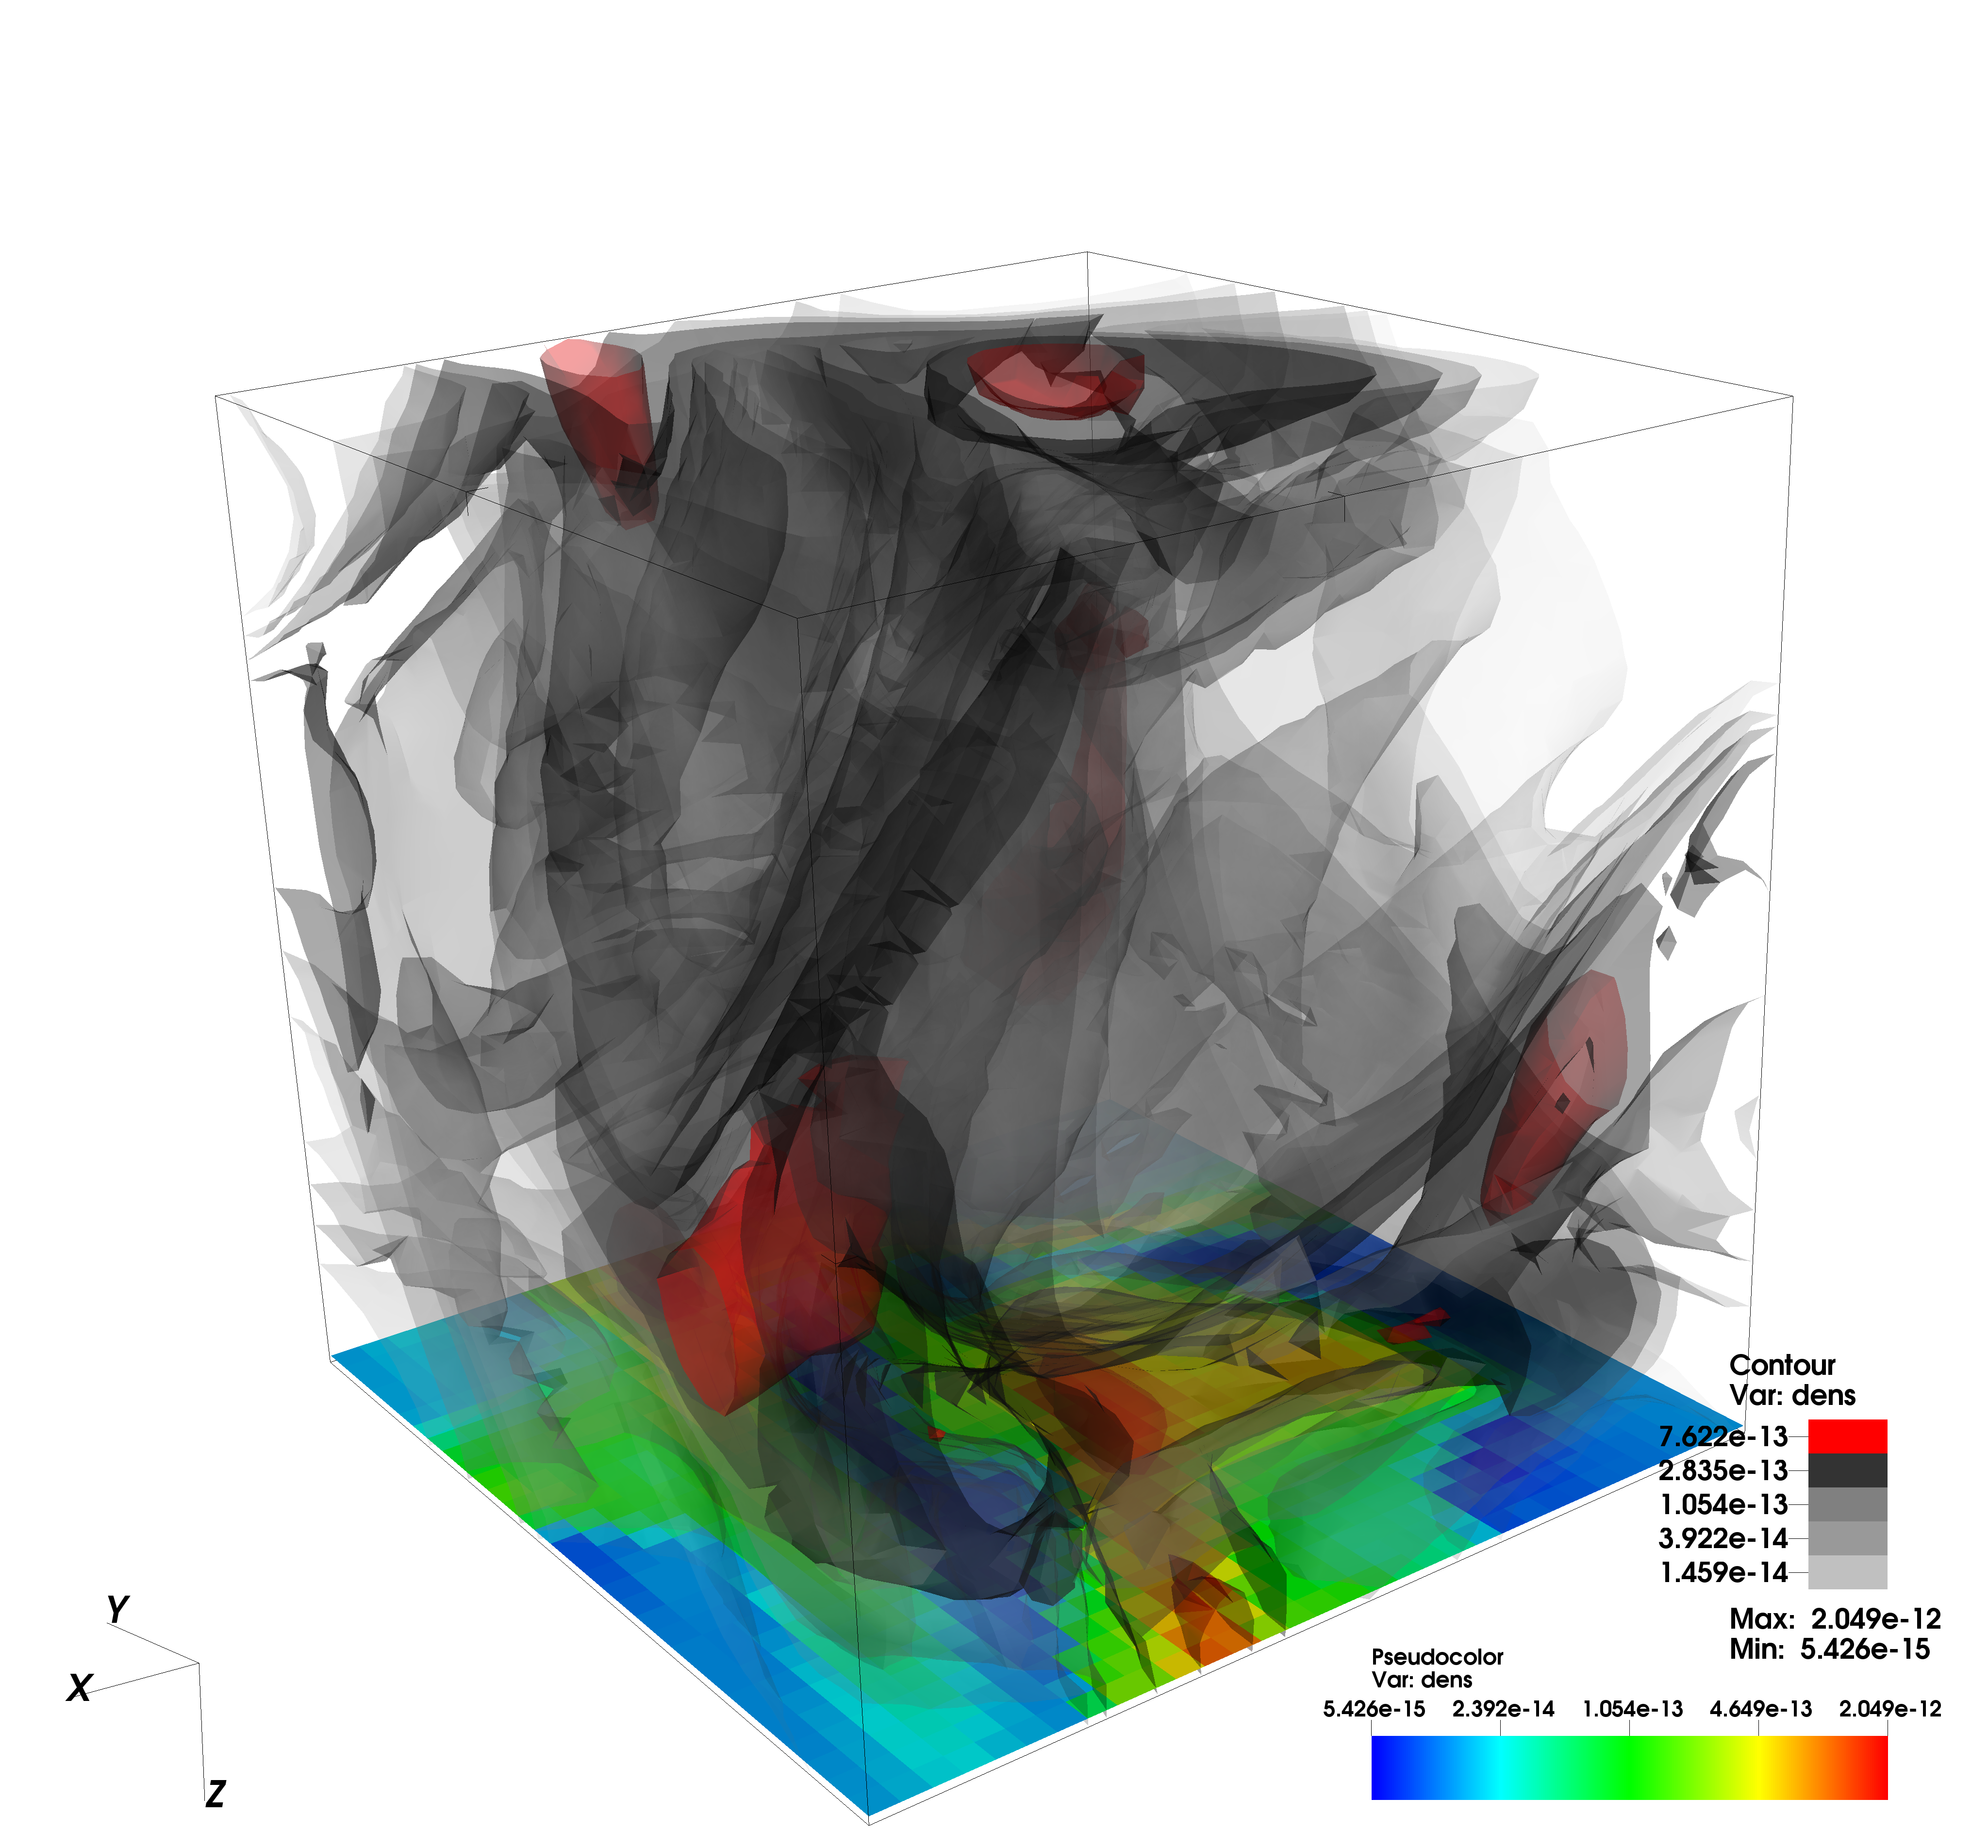
\includegraphics[height=5.5cm,clip=true]{Graphics/bbb_0375_dens_contour_00500000.png}%
	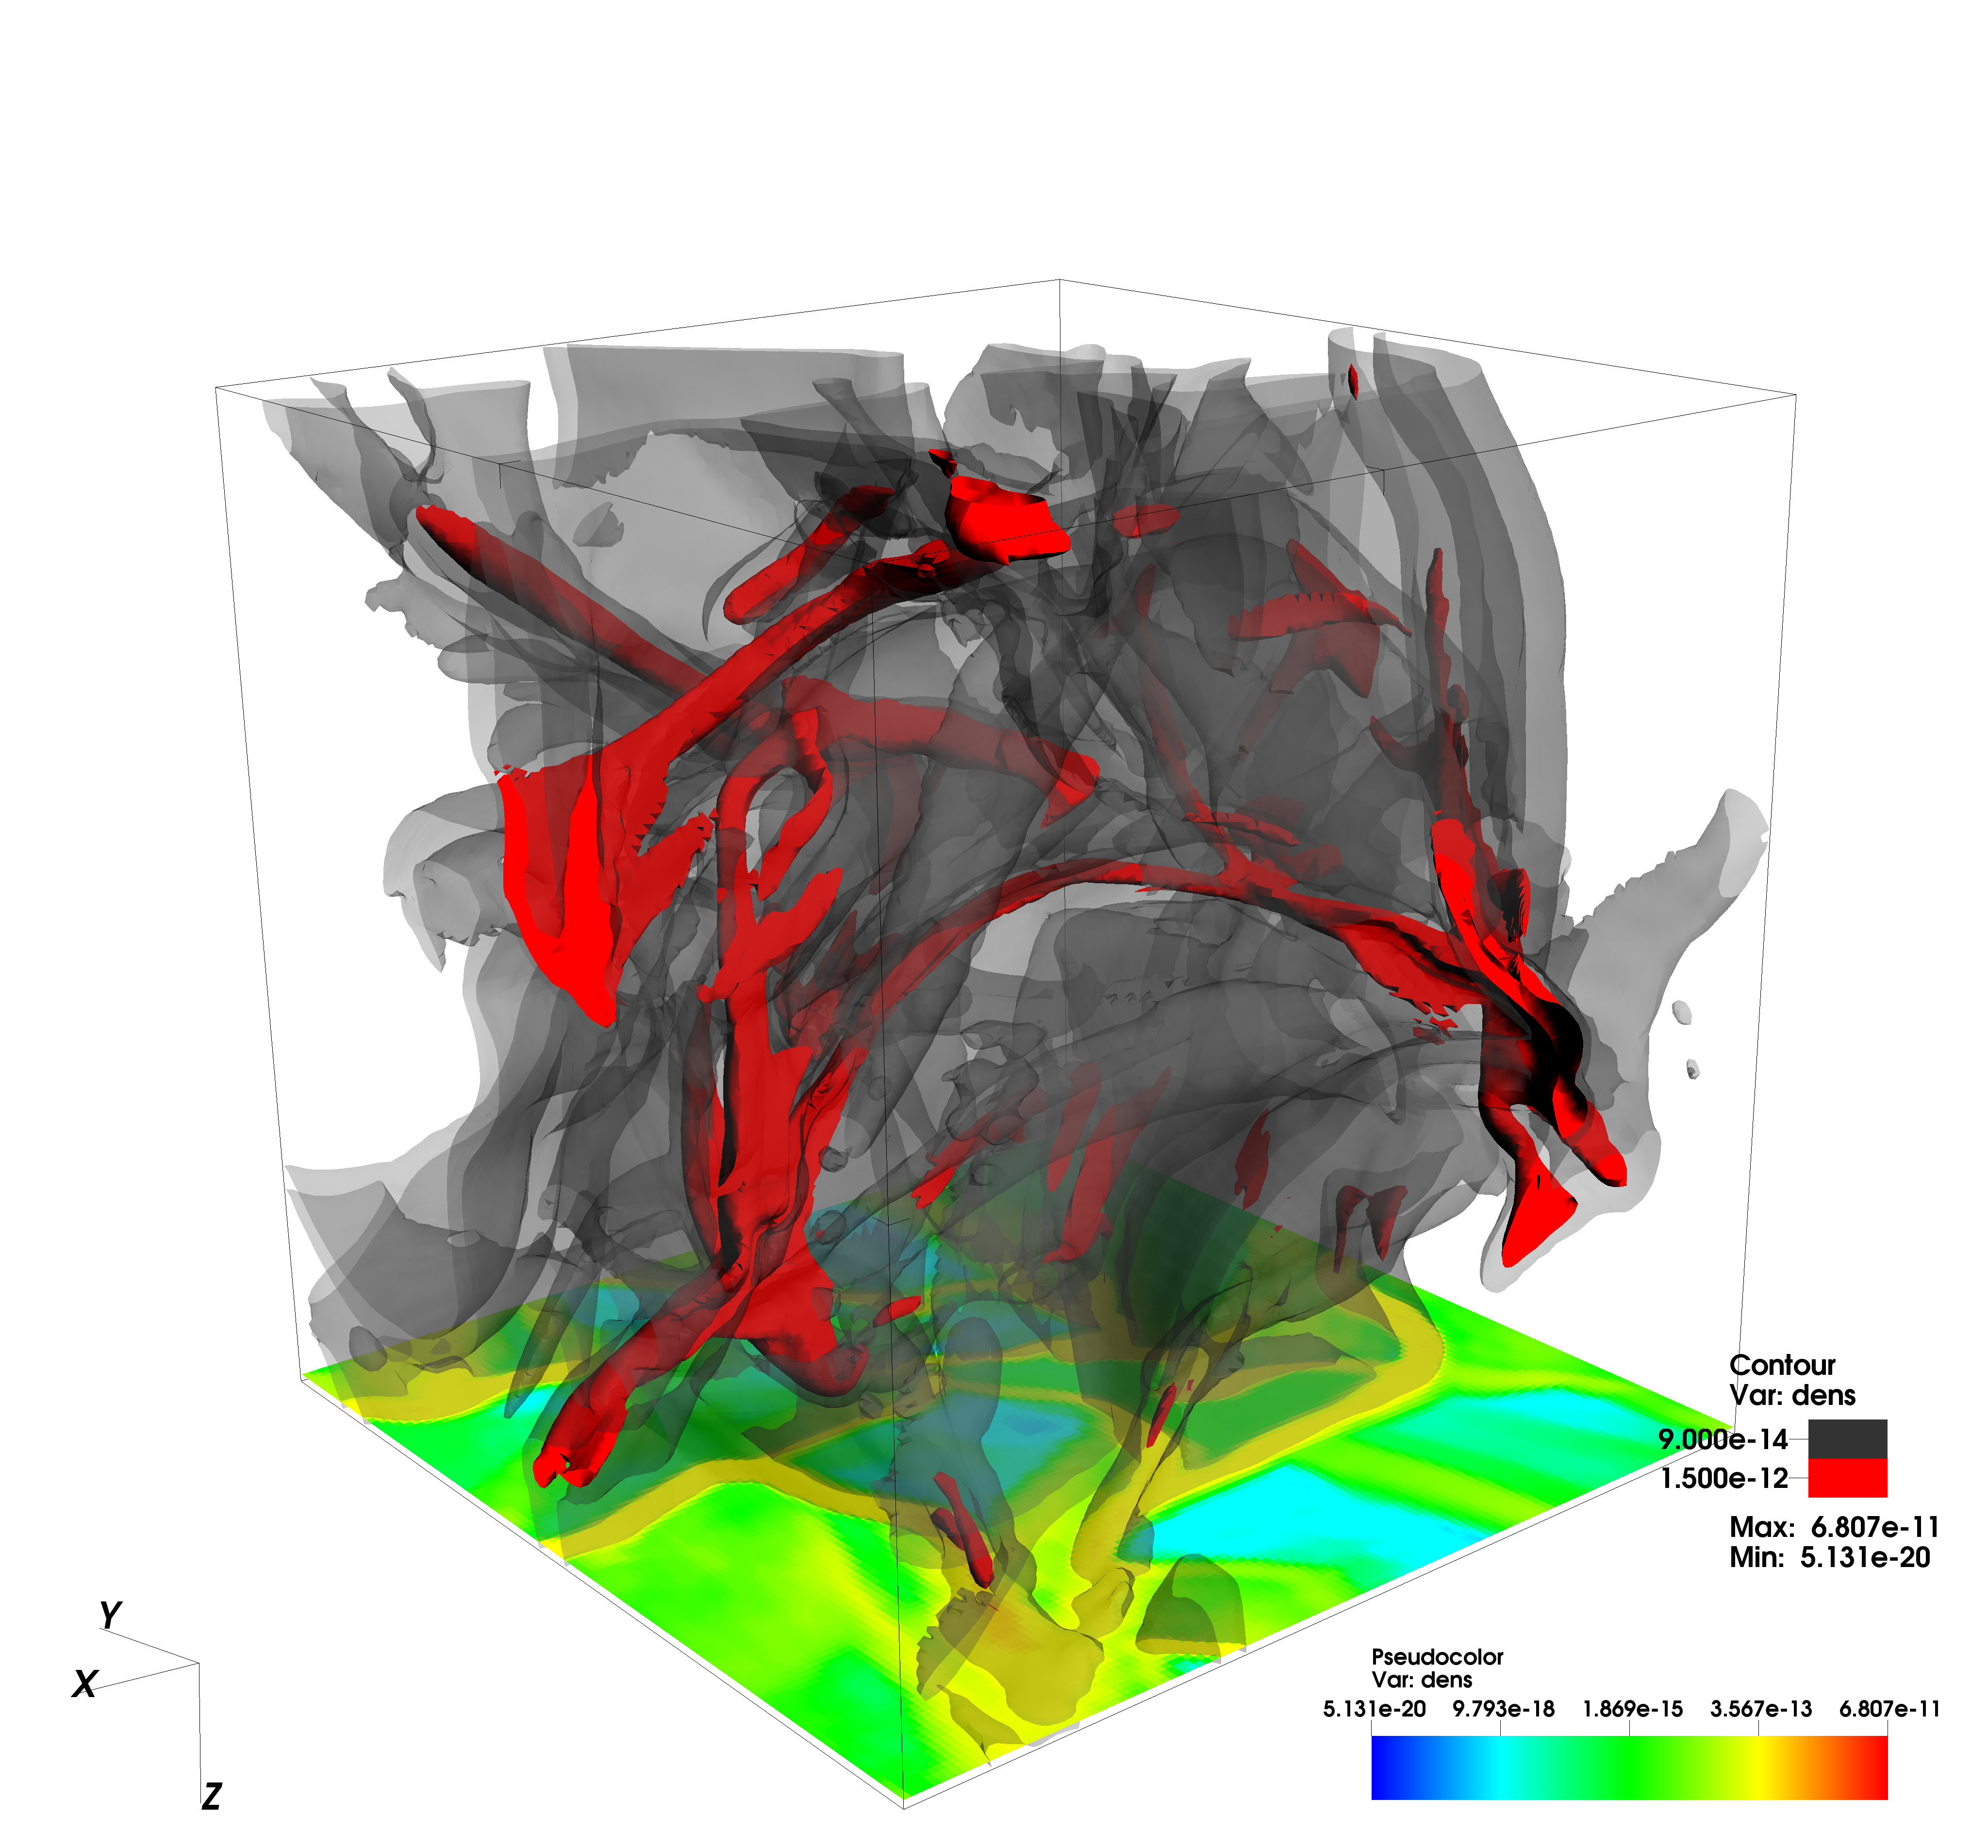
\includegraphics[height=5.5cm,clip=true]{Graphics/bbb_0375_dens_contour_0200_0002.png}%
	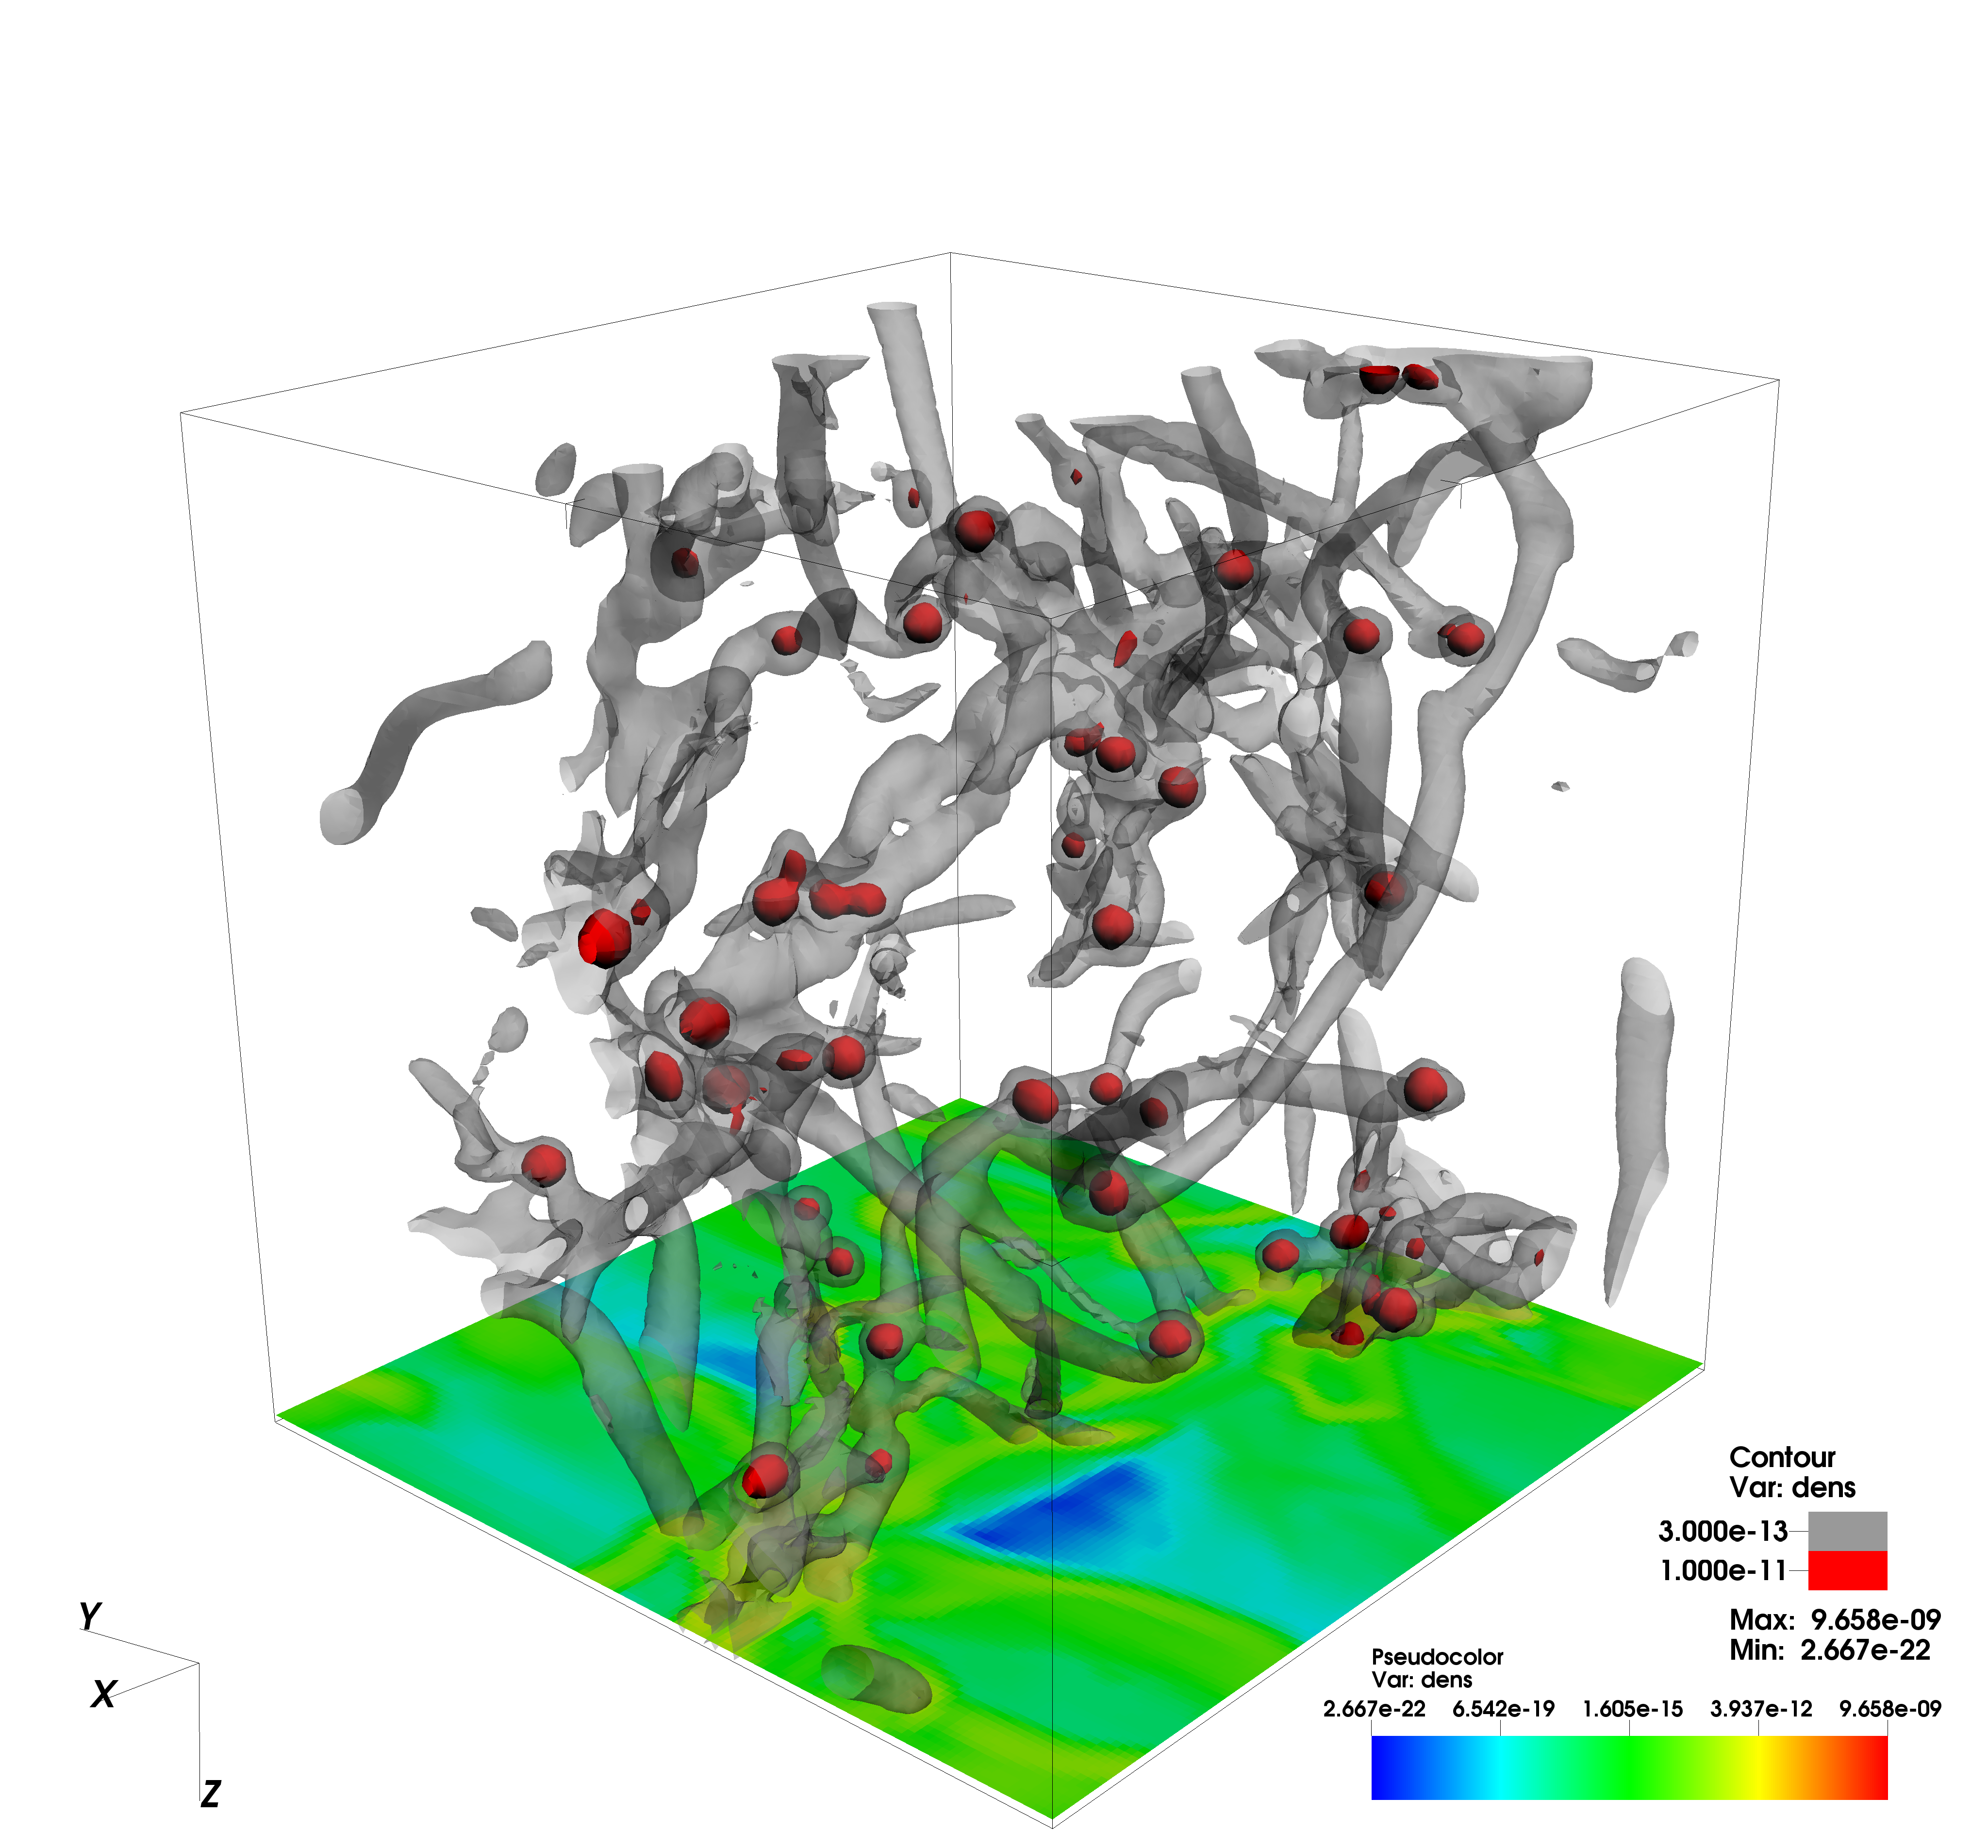
\includegraphics[height=5.5cm,clip=true]{Graphics/bbb_0375_dens_contour0000.png}
	\end{center}
	\caption{Evolution of a star-forming molecular cloud over time. The leftmost panel shows the density contour just after perturbation, with sheet-like structures most prominent. The middle panel shows the collapse of those sheets into filaments in the densest (red) regions. The rightmost panel shows a near-complete transition to filaments, and the densest (red) regions indicate the position of protostars.}
	\label{f:cloudevolution}
	\end{figure*}





\section{Methods}\label{Methods}

\subsection{Fractal analysis methods}\label{FractalMethods}
A box-counting algorithm (see, for example, \cite{Falconer2003}) was implemented in order to determine the fractal dimension of the flame front. With this algorithm we can describe the fractal dimension, $\mathrm{dim}$, as
\begin{equation}\label{dimensioneqn}
	\mathrm{dim}_B = \lim_{\epsilon \to 0} \frac{\log N(\epsilon)}{\log (1 / \epsilon)},
\end{equation}
where $N$ is the number of boxes containing the structure of interest.  To implement the estimation in Equation \ref{dimensioneqn}, one must introduce coarse-graining of the data under study. In the flame front analysis performed here, trilinear interpolation is performed in order to determine the location of the flame front within the coarse mesh. For each level of coarse-graining, $\log{N(\epsilon)}$ and $\log{(1/\epsilon)}$ is calculated, and a linear regression is performed on the four points with finest resolution in order to estimate the dimension as given in Equation \ref{dimensioneqn}.

\subsection{Multifractal analysis methods}\label{MultifractalMethods}
The multifractal spectrum of some set is the plot of $f(\alpha)$ vs. $\alpha$, where $f(\alpha)$ is the fractal dimension of the subset of all points with local density $\alpha$ (see \cite{Falconer2006}). To obtain the multifracta spectra we use the method of \cite{Chhabra1989}. We reparametrize both $f$ and $\alpha$ as functions of a moment exponent $q$ that serves to weight the features of the density on various scales. For every value of $q$, we define the normalized measure $\mu_i(q, \epsilon)$ of box $i$ with side length $\epsilon$ as
\begin{equation} 
	\mu_i(q, \epsilon) = \frac{[M_i(\epsilon)]^q}{\sum_j[M_j(\epsilon)]^q},
\end{equation}
where $M_i$ is the mass contained in each box $i$. Now we can express $f(\alpha)$ as
\begin{equation}
	f(q) = \lim_{\epsilon \to 0} \frac{\sum_i \mu_i(q, \epsilon) \log[\mu_i(q, \epsilon)]}{log \epsilon},
\end{equation}
and $\alpha$ as
\begin{equation}
	\alpha (q) = \lim_{\epsilon \to 0} \frac{\sum_i \mu_i(q, \epsilon) \log[M_i(\epsilon)]}{log \epsilon}.
\end{equation}


\subsection{Verification}\label{Verification}

Our implementation of the box-counting algorithm was verified against computer-generated data with known fractal characteristics. The implementation was able to recover the theoretical dimension with 10\% accuracy. \footnote{insert table of results here?}

This algorithm’s implementation was verified against a computer-generated multifractal system and produced the expected plot of $f(\alpha)$ vs. $\alpha$. \footnote{include graphic of IFS and binomial multifractal used for verification}

\section{Results}\label{Results}

\subsection{Fractal analysis}\label{FractalResults}
The method described above was applied to the contour shown in Figure \ref{f:flamefrontwithcontour}, and the fractal dimension of the contour was found to be 1.05. \cite{Timmes1994} and \cite{Blinnikov1996} estimated the fractal dimension of flame fronts in three dimensions to be between 2.3 and 2.6. Intuitively, then, one would expect the fractal dimension of a flame front in two dimensions to be between 1.3 and 1.6, a discrepancy we examine in \textsection \ref{Discussion}.

\begin{figure}
	\begin{center}
	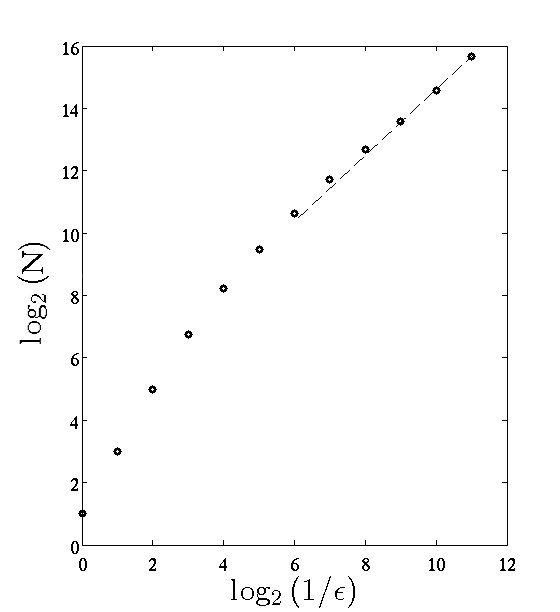
\includegraphics[width=0.45\textwidth,clip=true]{Graphics/logNvsE.png}
	\caption{Regression to find the fractal dimension of the flame contour shown in Figure \ref{f:flamefrontwithcontour}. The slope of the regression line indicates the fractal dimension—about 1.05.
	\label{f:logNvsE}}
	\end{center}
	\end{figure} 


\subsection{Multifractal analysis}\label{MultifractalResults}

\begin{figure}
	\begin{center}
	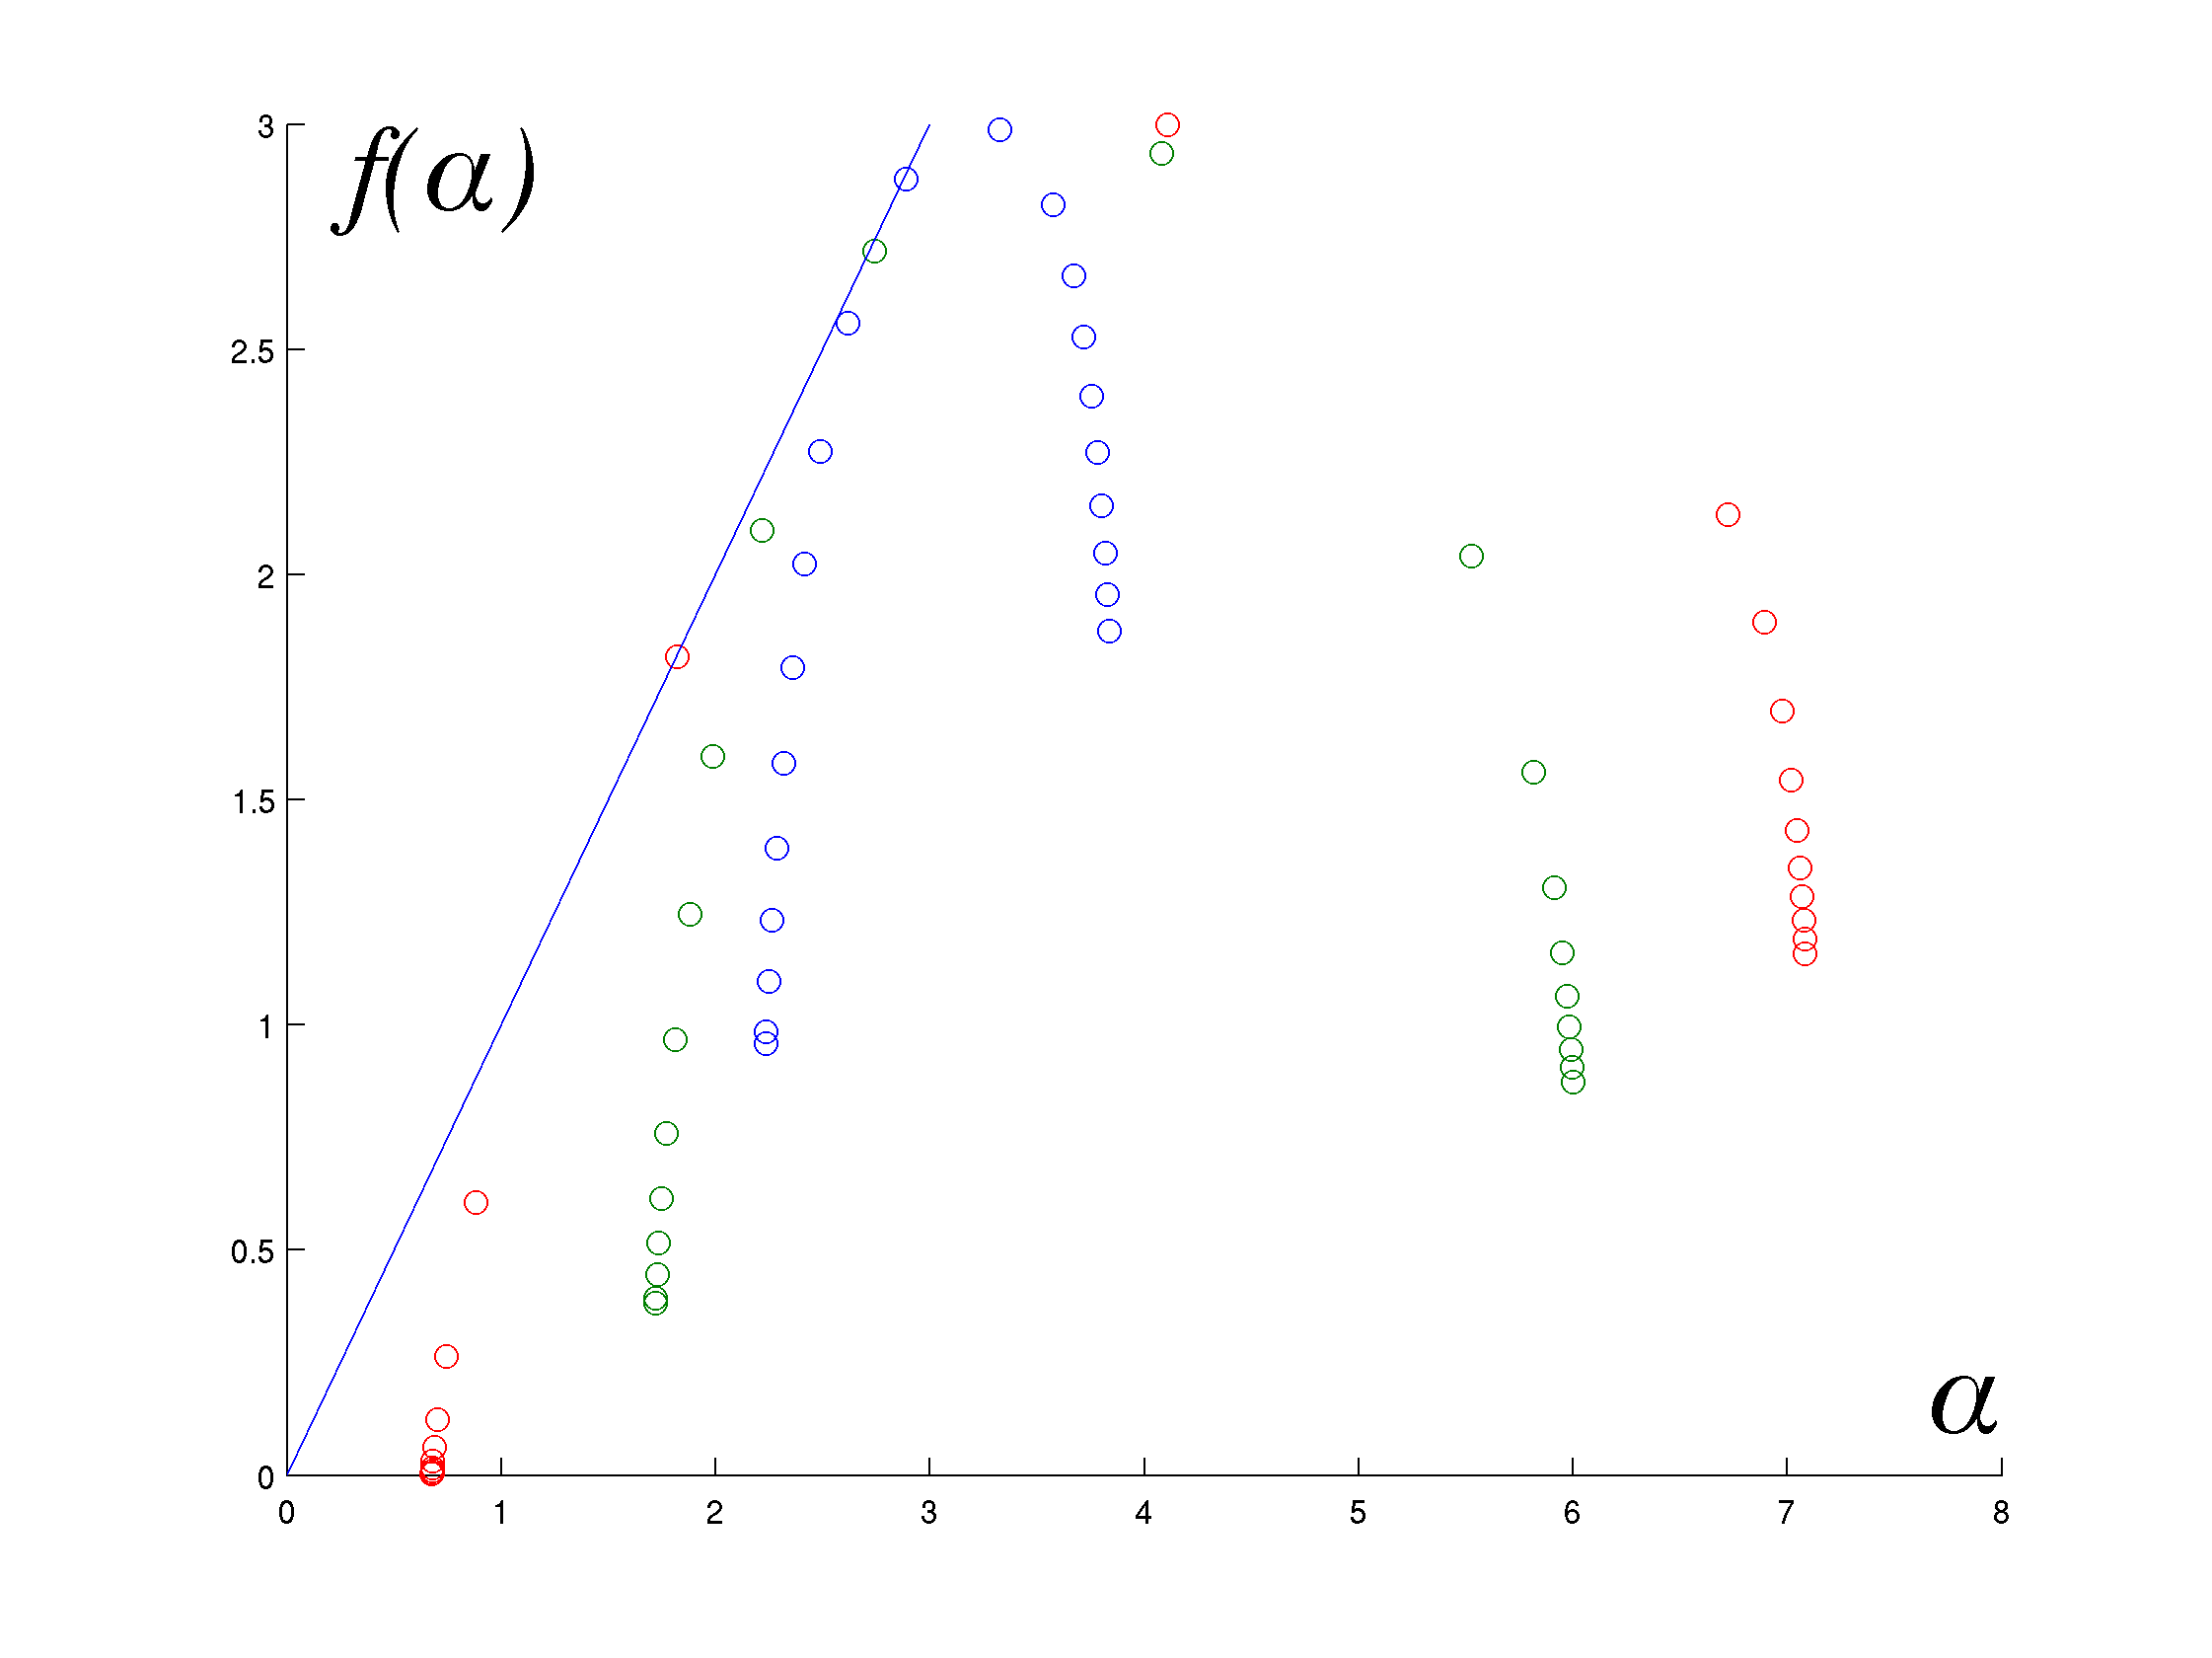
\includegraphics[width=0.45\textwidth,clip=true]{Graphics/falphaclouds.png}
	\caption{Plot of $f(\alpha)$ vs. $\alpha$ for the molecular cloud pictured in Figure \ref{f:cloudevolution}. The blue plot shows the spectrum of the earliest timestep (leftmost panel); the green plot shows the spectrum of the middle timestep (middle panel); and the red plot shows the spectrum of the last timestep (rightmost panel). The blue line $f(\alpha) = \alpha $ intersects the curves at the points where $f(\alpha)$ gives the dimension of the entire structure.
	\label{f:falphamultifractal}}
	\end{center}
	\end{figure} 

The multifractal spectra generated from the molecular cloud pictured in Figure \ref{f:cloudevolution} are presented in Figure \ref{f:falphamultifractal}. The blue plot shows the spectrum of the earliest timestep (leftmost panel); the green plot shows the spectrum of the intermediate timestep (middle pannel); and the red plot shows the spectrum of the last timestep (rightmost panel). The blue line $f(\alpha) = \alpha $ intersects the curves at the points where $f(\alpha)$ gives the dimension of the entire structure \citep{mandelbrotmultifractal}. Each curve has a maximum at $f(\alpha) \approx 3$, occurring when the moment exponent $q = 0$. This maximum, then, can be interpreted as the dimension of the space in which the cloud lies \citep{Schroeder}, so a dimension of 3 is to be expected. 

\section{Discussion}\label{Discussion}
Possible causes for the discrepancy between the dimension of the flame front found here and the values cited include the coarseness of the model used and the large differences in the character of 2D and 3D turbulence. Still, a robust implementation was developed that can investigate this discrepancy further and handle any uniform-meshed data.
 
The narrowing of the spectra in the molecular cloud studied agrees with our expectations: as the system evolves, it exhibits a narrower range of scaling exponents $ \alpha $ during its transition from a structure that is partly sheet-like to one that clearly resembles filaments. In addition, the points that intersect the blue line in Figure \ref{f:falphamultifractal} decrease from a dimension of just below 3 (where the structure is primarily sheet-like) to about 2.7 (in the intermediate state) to about 1.7 (when the collapsed filaments have formed).

%--------------------
%	Begin ackownledgements
%--------------------
\section{Acknowledgments}\label{s:ack}
The author would like to thank Dr. Tomasz Plewa and Tim Handy for their guidance and support, as well as the Young Scholars Program at Florida State University for the opportunity to conduct this research.
%
%
%--------------------
%	Begin references
%--------------------
\bibliographystyle{apj}
\bibliography{main}
%
%
%

\end{document}
